% !TeX spellcheck = en_US
% !TeX encoding = UTF-8
\documentclass[aps, 11pt, a4paper]{article}
\usepackage{graphics, graphicx, graphics}
\usepackage{fancyvrb, enumerate}
\usepackage{amsmath, amssymb, amscd, amsfonts}
\usepackage{geometry}
\usepackage{multirow}
\usepackage{url}
\usepackage{tikz}
\usepackage{listings, listing}
\usepackage{color}
\usepackage{mathptmx}

\usetikzlibrary{shapes, arrows, calc, positioning}
\definecolor{codegreen}{rgb}{0, 0.6, 0}
\definecolor{codegray}{rgb}{0.5, 0.5, 0.5}
\definecolor{codepurple}{rgb}{0.58, 0, 0.82}
\definecolor{backcolour}{rgb}{0.95, 0.95, 0.92}
\lstdefinestyle{mystyle}
{
    backgroundcolor=\color{backcolour},   
    commentstyle=\color{codegreen},
    keywordstyle=\color{magenta},
    numberstyle=\tiny\color{codegray},
    stringstyle=\color{codepurple},
    basicstyle=\footnotesize,
    breakatwhitespace=false,         
    breaklines=true,                 
    captionpos=b,                    
    keepspaces=true,                 
    numbers=left,                    
    numbersep=5pt,                  
    showspaces=false,                
    showstringspaces=false,
    showtabs=false,                  
    tabsize=2,
    frame=single
}
\lstset{style=mystyle}
\tikzstyle{decision} = [diamond, draw, fill=blue!20, text width=4.5em, text badly centered, node distance=3cm, inner sep=0pt]
\tikzstyle{block} = [rectangle, draw, fill=blue!20, text width=5em, text centered, rounded corners, minimum height=2em]
\tikzstyle{line} = [draw, -latex']
\tikzstyle{cloud} = [draw, ellipse, fill=red!20, node distance=5em, minimum height=2em]
\tikzset
{
    -|-/.style=
    {
        to path=
        {
            (\tikztostart) -| ($(\tikztostart)!#1!(\tikztotarget)$) |- (\tikztotarget)
            \tikztonodes
        }
    },
    -|-/.default=0.5,
    |-|/.style=
    {
        to path=
        {
            (\tikztostart) |- ($(\tikztostart)!#1!(\tikztotarget)$) -| (\tikztotarget)
            \tikztonodes
        }
    },
    |-|/.default=0.5,
}
\geometry
{
    top = 20mm,
    bottom = 20mm,
    left = 20mm,
    right = 20mm
}

\title{Prediction for Periodontists by Oral Bacteria in Korean\\ \large 2020 1st Semester Interdisciplinary Project}
\author{20161206 JaewoongLee}
\date{\today}

\begin{document}
    \maketitle
    \begin{table}[h]
    	\centering
		\begin{tabular}{c|c}
			Student ID & 20161206 \\ \hline
			Name & Jaewoong Lee \\ \hline
			School & School of Electrical \& Computer Engineering \\ \hline
			1 Track & Computer Science \& Engineering \\ \hline
			2 Track & Bio-medical Engineering \\ \hline
			Advisor 1 & Sungahn Ko \\ \hline
			Advisor 2 & Semin Lee \\
		\end{tabular}
    \end{table}
    \newpage
    
    \tableofcontents
    \listoftables
    \listoffigures
    \newpage
    
    \section{Introduction}
    	\subsection{Periodontitis}
    		Periodontitis is an inflammatory disease of the periodontium which is characterized by a progressive destruction of the tissues supporting the tooth \cite{ref:perio2}. In histopathologically, periodontitis may result periodontal pocketing, location of junctional epithelium apical to the cemento-enamal junction, loss of collagen fibers subjacent to the pocket epithelium, numerous poly-morphonuclear leukocytes in epithelium and a dense inflammatory cell infiltrate with plasma cells, lymphocytes, and macrophages \cite{ref:perio1}. Periodontits is currently assumed to progress as periodic, relatively short episodes of rapid tissue destruction followed by some prolonged intervening periods of disease remission \cite{ref:perio2}. 
    		
    		\begin{figure}[htbp]
    			\centering
    			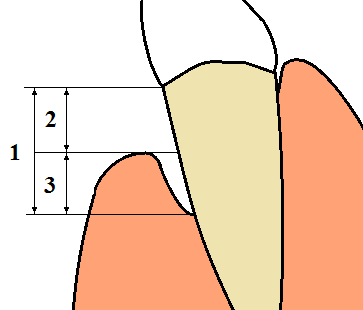
\includegraphics[width=0.3 \linewidth]{figures/recession.png}
    			\caption{Diagram of Gingival Recession \protect \cite{ref:depth1}}
    			\label{fig:depth}
    		\end{figure}
    	
    		Periodontitis is diagnosed by measuring clinical attachment loss (CAL). Note that the CAL is the length of the figure \ref{fig:depth}-1, which is sum of gingival recession (figure \ref{fig:depth}-2) and probing depth (figure \ref{fig:depth}-3).
    		
    		Periodontitis is generally believed to be a result of a host-parasite interaction in which bacteria are the determinants of periodontitis \cite{ref:cause1}. In etiology, the primary cause of periodontitis is presumed as a bacterial infection as the primary cause of periodontitis \cite{ref:perio1}. Thus, the treatment of periodontitis includes antibiotics and dental surgery.
    		
    		In this manner, some medicines have been introduced for treatment. However, the success in the prevention and treatment of periodontitis has been limited. Many \textit{in vitro} studies shows that Asian have the different bacteria from non-Asian, due to their groceries \cite{ref:asian1}. Thus, the developments of plaque and calculus in Asian differ, and may lead to distant reactions between Asian and non-Asian.
    		
    	\subsection{Machine Learning}
    		Machine learning is the study of algorithms which advance spontaneously through experience. Machine learning is conjugated where is infeasible with conventional algorithms such as computer vision.  Many papers show that machine learning brings out better result than human recognition. 
    	
    		If the feedback provides the correct answer for specific inputs, then learning problem is called supervised learning \cite{ref:ai1}. Classification is a kind of supervised learning for discrete values; regression is for continuous values.
    		
    	\subsection{Purpose of Research}
    		There are many studies which have tried to find bacteria as bio-markers \cite{ref:biomarker1, ref:biomarker2}. 
    		
    		Hence, the purposes of this research are as:
    		\begin{enumerate}
				\item Classify the stage of periodontitis by oral bacteria.
				\item Regress the CAL, gingival recession, or probing depth by oral bacteria. 
    		\end{enumerate}
    
    \section{Materials}
    
    \section{Methods}
    	\subsection{Python Packages}
    		Python programming language had been used to analyze data. Also, many Python modules had been adopted as hereinafter.
    		
    		\subsubsection{Pandas}
    		\textit{Pandas} is a Python library of rich data structures and tools for working with structured data sets common to statistics, finances, social sciences, and many other fields \cite{ref:pandas1}.
    		
    		\subsubsection{Scikit-learn: Machine Learning in Python}
    			\textit{Scikit-learn} is a Python module integrating a wide range of state-of-the-art machine learning algorithms for medium-scale supervised and unsupervised problems \cite{ref:sklearn1}. Also, the following algorithms amongst \textit{Scikit-learn} package are used:
    			\begin{itemize}
					\item AdaBoost
					\item Adam Neural Network
					\item DecisionTree
					\item K-Neighbors
					\item LBFGS Neural Network
					\item Linear SVC
					\item Poly SVC
					\item Random Forest
					\item RBF SVC
					\item Sigmoid SVC
    			\end{itemize}
    			    			
    		\subsubsection{Seaborn}
		   		\textit{Seaborn} is a Python data visualization library based on \textit{matplotlib}. It provides a high-level interface for drawing attractive and informative statistics graphics \cite{ref:seaborn1}.

    			
    	\subsection{Stages of Periodontitis}
    		There are five clinical stages of periodontitis:
    		\begin{enumerate}
				\item Healthy
				\item Slight
				\item Moderate
				\item Severe
				\item Acute
    		\end{enumerate}
    
    \section{Results}
    
    \section{Discussion}
    
    \section{Acknowledgment}
    
    \addcontentsline{toc}{section}{References}
    \bibliographystyle{IEEEtran}
    \bibliography{reference}
\end{document}